\chapter{本テンプレートの使い方}
\label{chap:howto}

本章では、本テンプレートの具体的な使用方法を解説する。基本的には、{\tt main.tex} を上から順に修正していけばよいだけ。 


\section{テンプレートの構成}

このテンプレートは、表\ref{tb:files}のファイルで構成されている。

\begin{table}[htbp]
  \caption{構成ファイル}
  \label{tb:files}
  \begin{center}\begin{tabular}{c|l}
    \hline
    ファイル名&用途\\\hline\hline
    {\tt main.tex}&メインのファイル。これを編集していく\\\hline
    {\tt thesis.sty}&論文のスタイルを定義したファイル。基本的には手は加えない\\\hline
    {\tt *.tex}&{\tt main.tex}に{\tt include}されるファイル群\\\hline
    {\tt *.eps}&画像ファイル\\\hline
    {\tt main.bib}&参考文献用のBibTeXファイル\\\hline
    {\tt Makefile}&Makefile。次節以降で説明\\\hline
    {\tt .gitignore}&Git用設定ファイル\\\hline
  \end{tabular}\end{center}
\end{table}

\section{コンパイル}
このテンプレートの\LaTeX ファイルをコンパイルしてPDFファイルを生成するには、ターミナルを開いて以下のようにする。

\begin{itembox}[l]{コマンド実行例}
\begin{verbatim}
% make
\end{verbatim}
\end{itembox}

こうすることで、\verb|platex|コマンド、\verb|pbibtex|コマンド、\verb|platex|コマンド2回、\verb|dvipdfmx|コマンドが全て実行され、{\tt main.pdf}が生成される。

コンパイルによって生成されたファイルを全て消すには、以下のようにする。

\begin{itembox}[l]{コマンド実行例}
\begin{verbatim}
% make clean
\end{verbatim}
\end{itembox}

\section{設定}

以下、{\tt main.tex}に対して行うべき設定を、このファイルの中に書いてある順に沿って説明する。

\subsection{論文全体の言語の設定}
\label{sec:lang}

\begin{itembox}[l]{{\tt main.tex}}
\begin{verbatim}
\japanesetrue	% 論文全体を日本語で書く(英語で書くならコメントアウト)
\end{verbatim}
\end{itembox}

ここでは論文全体の言語を設定する。日本語に設定すれば、『章』『目次』『謝辞』などが日本語で出力されて、行頭のインデントなども日本語の仕様になる。英語にした場合は、これらはそれぞれ『Chapter』『Table of Contents』『Acknowledgment』な体裁になる。インデントも行間も、英語用の設定が適用される。

\verb|\japanesetrue| をコメントアウトしなければ日本語に、コメントアウトすれば英語に設定される。


\subsection{余白の設定}

\begin{itembox}[l]{{\tt main.tex}}
\begin{verbatim}
\bindermode	% バインダ用余白設定
\end{verbatim}
\end{itembox}

このテンプレートの出力はA4用紙。ここではこれの四辺の余白を設定する。

最終的にバインダーで綴じて提出する場合、余白を左右対称にしてしまうと、見かけ上のバランスがとても悪くなる。これを解消するため、あらかじめ左側の余白を大きく取っておく。

\verb|\bindermode| をコメントアウトしなければ左綴じ用の余白に、コメントアウトすれば左右対称の余白に設定される。

両面印刷の場合、偶数ページと奇数ページで余白を広くとるべき側が違うので、\verb|documentclass| でこれを設定する。

\begin{itembox}[l]{{\tt main.tex}}
\begin{verbatim}
% 両面印刷の場合。余白を綴じ側に作って右起こし。
\documentclass[a4j,twoside,openright,11pt]{jreport}
% 片面印刷の場合。
%\documentclass[a4j,11pt]{jreport}
\end{verbatim}
\end{itembox}

両面印刷の場合は \verb|twoside| を使用する。\verb|openright| を使うと章のはじまりが必ず右側のページに来るようになる。

\subsection{論文情報の設定}
\label{sec:meta}

\begin{itembox}[l]{{\tt main.tex}}
\begin{verbatim}
% 日本語情報(必要なら)
\jclass  {修士論文}                             % 論文種別
\jtitle    {修士論文用 \LaTeX\ テンプレート}    % タイトル。改行する場合は\\を入れる
\juniv    {慶應義塾大学大学院}                  % 大学名
\jfaculty  {政策・メディア研究科}               % 学部、学科
\jauthor  {ほげ山 ふう助}                       % 著者
\jhyear  {24}                                   % 平成○年度
\jsyear  {2012}                                 % 西暦○年度
\jkeyword  {\LaTeX、テンプレート、修士論文}     % 論文のキーワード
\jproject{インタラクションデザインプロジェクト} %プロジェクト名
\jdate{2013年1月}

% 英語情報(必要なら)
\eclass  {Master's Thesis}                            % 論文種別
\etitle    {A \LaTeX Template for Master Thesis}      % タイトル。改行する場合は\\を入れる
\euniv  {Keio University}                             % 大学名
\efaculty  {Graduate School of Media and Governance}  % 学部、学科
\eauthor  {Fusuke Hogeyama}                           % 著者
\eyear  {2012}                                        % 西暦○年度
\ekeyword  {\LaTeX, Templete, Master Thesis}          % 論文のキーワード
\eproject{Interaction Design Project}                 %プロジェクト名
\edate{January 2013}
\end{verbatim}
\end{itembox}

ここでは論文のタイトルや著者の氏名などのメタデータを記述する。ここで書いたデータは、表紙とアブストラクトのページに使われる。必ずしも日本語と英語の両方を設定しなければいけないわけではなくて、自分が必要とする方だけ記述すればよい。

タイトルが長過ぎる場合は、表紙やアブストラクトのページでは自動で折り返して出力される。もし改行位置を自分で指定したい場合は、その場所に \verb|\\| を入力する。


\section{出力}

\verb|\begin{document}| から \verb|\end{document}| に記述した部分が、実際に{\tt DVI}(最終的には{\tt PDF})ファイルとして出力される。

\subsection{外部ファイルの読み込み({\tt include})}

出力部分の具体的な説明の前に、外部ファイルを読み込む方法を説明する。

\verb|\begin{document}| から \verb|\end{document}| の間では、\verb|\include| コマンドを使うことで、別の {\tt *.tex} ファイルを読み込ませられる。 

\begin{itembox}[l]{{\tt include}しない場合}
\begin{itembox}[l]{{\tt main.tex}}
\begin{verbatim}
\begin{document}
  \begin{jabstract}
  ほげほげ
  \end{jabstract}
\end{document}
\end{verbatim}
\end{itembox}
\end{itembox}

\begin{itembox}[l]{{\tt include}する場合}
\begin{minipage}{0.5\hsize}
\begin{itembox}[l]{{\tt main.tex}}
\begin{verbatim}
\begin{document}
\chapter{序論}
\label{chap:introduction}

本章では,本研究の背景と本論文の構成について述べる.

\newpage

\section{背景}

Webブラウザ上での情報検索が近年広く利用されている.

我々は普段情報検索を行う際,古い情報よりも新しい情報を求めていることが多いと考えられる.つまり古い情報よりも新しい情報の方が価値が高いのである.

しかし,Web 検索の結果一覧画面における各情報は,実世界に存在する紙やインクのように時間経過による外見的な劣化がないため,情報の鮮度を直感的に判断するのは難しい.

\begin{figure}[htbp]
  \begin{minipage}{0.5\hsize}
    \begin{center}
      \fbox{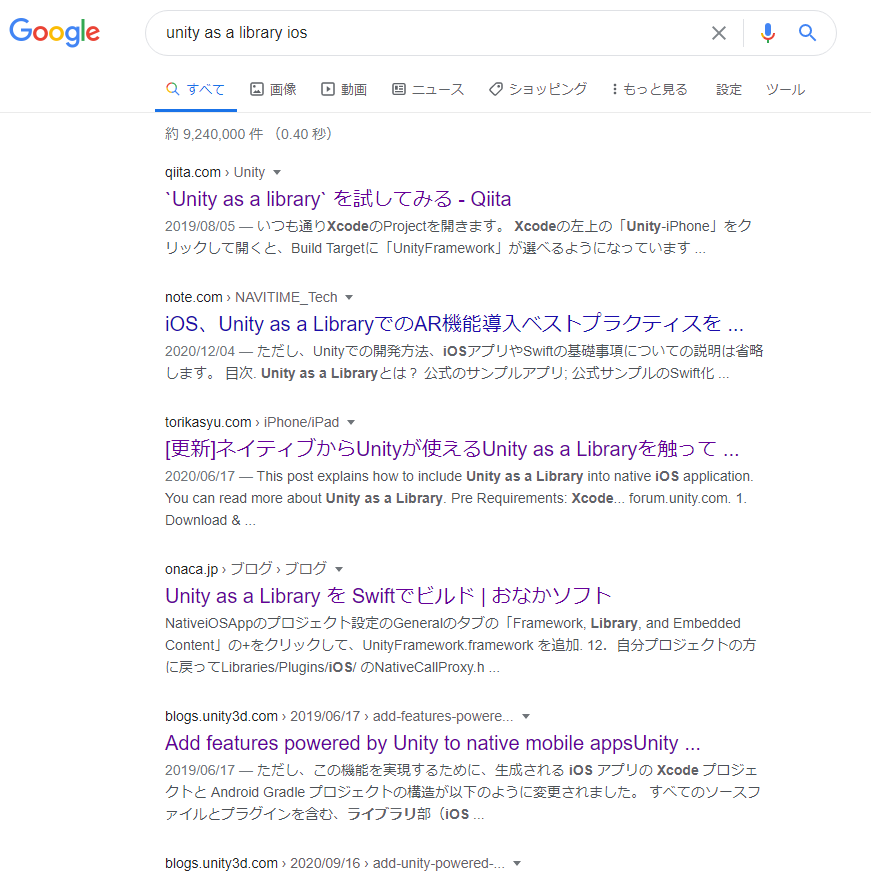
\includegraphics[width=60mm]{images/search-google.png}}
    \end{center}
    \caption{Google の検索結果一覧画面}
  \end{minipage}
  \begin{minipage}{0.5\hsize}
    \begin{center}
      \fbox{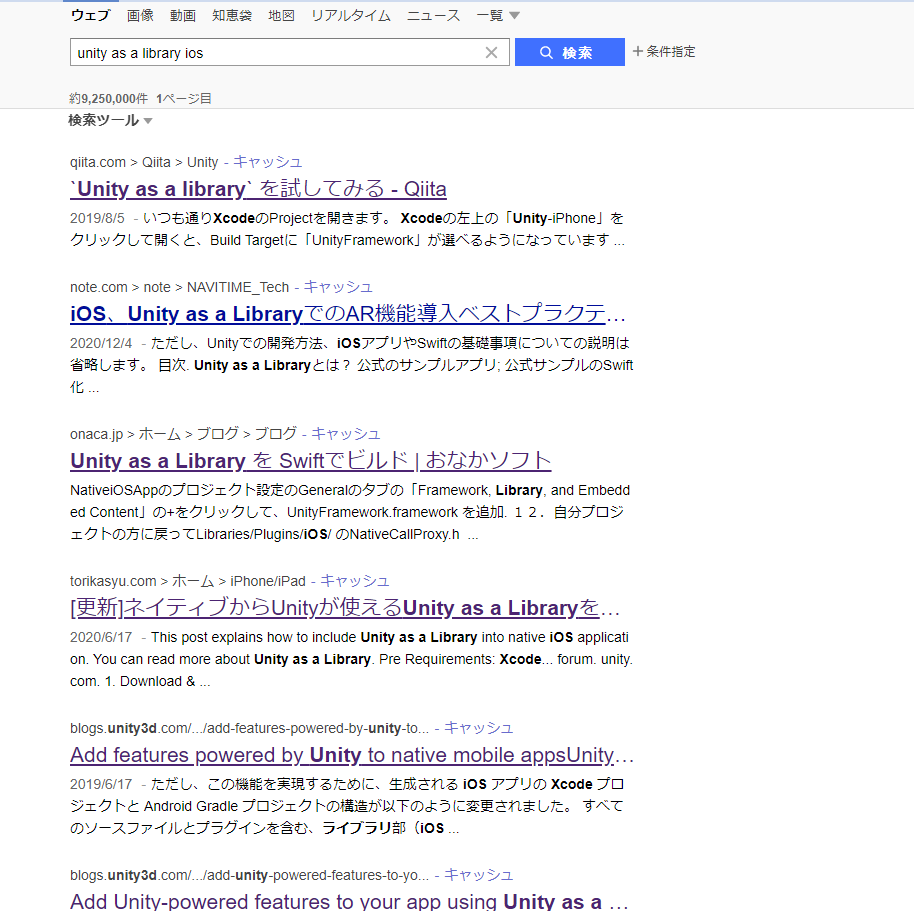
\includegraphics[width=60mm]{images/search-yahoo.png}}
    \end{center}
    \caption{Yahoo! の検索結果一覧画面}
  \end{minipage}
\end{figure}
\begin{figure}[htbp]
  \begin{minipage}{0.5\hsize}
    \begin{center}
      \fbox{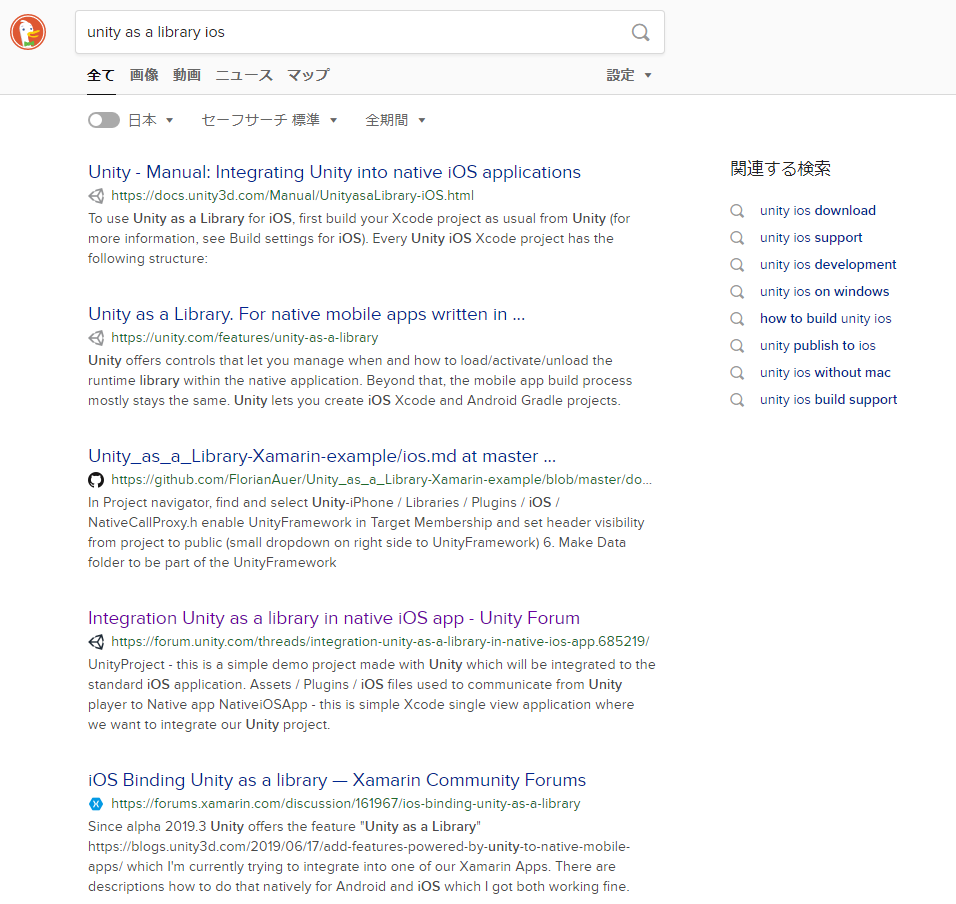
\includegraphics[width=60mm]{images/search-ddg.png}}
    \end{center}
    \caption{DuckDuckGo の検索結果一覧画面}
  \end{minipage}
  \begin{minipage}{0.5\hsize}
    \begin{center}
      \fbox{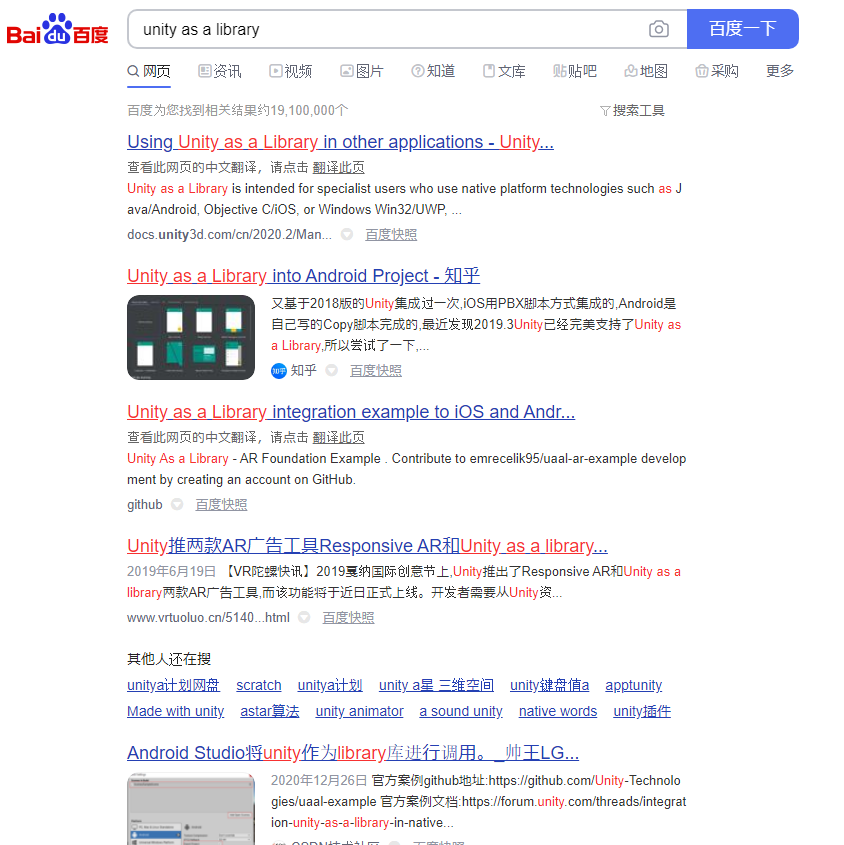
\includegraphics[width=60mm]{images/search-baidu.png}}
    \end{center}
    \caption{Baidu の検索結果一覧画面}
  \end{minipage}
\end{figure}

そこで,本来外見的な劣化のない各情報に,時間経過による表示の変化を与える.これにより情報の鮮度を直感的に認識できるようになり,Web 検索による情報収集を効率的に行えると考えた.

% こういった Web 検索結果一覧画面での情報の視覚化に関して,松下らは「ネット上の情報を可視化する技術」\cite{tecvisinfo}で,

% \begin{quote}
%   Web の規模が膨大になるにつれ,ランキングの精度がますます大きな問題となるが,精度向上にも限界があるため,情報可視化システムにかかる期待も今後大きくなると予想される.
% \end{quote}

% と述べている.

% また,ユーザが検索結果から最初の選択をするまでにかける時間が平均5.7秒だという調査\cite{pinball}があり,この短い時間でユーザに情報の鮮度を認識させなければならない.

リンク先のページの鮮度に応じてリンクの表現を変化させる「廃れるリンク」\cite{dyinglink}のようなシステムも存在するが,リンクのみへの適用であるため鮮度の表現方法に改善の余地があると考えた.

\section{本研究の目的}

本研究の目的は,ユーザがより直感的に情報の鮮度を認識できるように,ブラウザにおける検索結果一覧画面の表示を拡張することである.

\section{本文書の構成}

第\ref{chap:introduction}章では本研究における背景と目的について述べる.

第\ref{chap:verification}章では実際に視覚化システムを開発する前に様々な視覚化の方法を試し評価する.

第\ref{chap:implementation}章で開発したシステムの実装に関して述べ,第\ref{chap:discussion}章では実際に利用して得られた評価や今後の展望について述べる.

第\ref{chap:survey}章では本研究と関連のある研究事例を紹介している.第\ref{chap:conclusion}章では本研究を総括して結論を述べる.
 % 01.texをinclude
\end{document}
\end{verbatim}
\end{itembox}
\end{minipage}
\begin{minipage}{0.5\hsize}
\begin{itembox}[l]{{\tt 01.tex}}
\begin{verbatim}
\begin{jabstract}
ほげほげ
\end{jabstract}
\end{verbatim}
\end{itembox}
\end{minipage}
\end{itembox}

{\tt include}しない場合とする場合を比較するとこのとおり。どちらも出力結果は一緒。{\tt include}する場合は、読み込ませたい箇所に、読み込ませたい{\tt *.tex}ファイルの名前を、拡張子を除いて \verb|\include| コマンドで書けばよい。

\verb|\include| コマンドを用いるか用いないかは、たぶん文書量や個人の好みに依る。例えば章ごとに別のファイルにしておけば、修正箇所を探すときの手間が多少は省けるかもしれない。Gitで人と共有しつつ校正を頼むときにもファイルが分かれていたほうがコンフリクトを起こしにくい。


\subsection{表紙の出力}

\begin{itembox}[l]{{\tt main.tex}}
\begin{verbatim}
\ifjapanese
  \jmaketitle    % 表紙(日本語)
\else
  \emaketitle    % 表紙(英語)
\fi
\end{verbatim}
\end{itembox}

最初に、表紙を出力する。

\verb|\jmaketitle| が実行されると日本語の表紙が、\verb|\emaketitle| が実行されると英語の表紙がそれぞれ出力される。日本語の表紙には、第\ref{sec:meta}節で設定したうちの日本語の情報が、英語の表紙には同節で設定したうち英語の情報が、それぞれ参照されて、表記される。

デフォルトでは第\ref{sec:lang}説で設定した言語の表紙のみが出力されるようになっている。

\subsection{アブストラクトの出力}

\begin{itembox}[l]{{\tt main.tex}}
\begin{verbatim}
% ■ アブストラクトの出力 ■
%	◆書式:
%		begin{jabstract}〜end{jabstract}	:日本語のアブストラクト
%		begin{eabstract}〜end{eabstract}	:英語のアブストラクト
%		※ 不要ならばコマンドごと消せば出力されない。



% 日本語のアブストラクト
\begin{jabstract}

本論文では、Web 上の情報検索における検索結果一覧画面でそれぞれの情報の鮮度が一目で分かるシステムを提案する。

一般的な Web ブラウザでは、検索した情報がいつ公開されたかに応じて表示に差を設けることはしていないが、情報の取捨選択において情報の鮮度は重要な要素の一つである。

そこで、情報の表示に実世界における情報媒体が劣化していくメタファを適用することで、ユーザが検索した情報の鮮度をより直感的に認識することができる。

\end{jabstract}
	% アブストラクト。要独自コマンド、include先参照のこと
\end{verbatim}
\end{itembox}

表紙の次は、アブストラクト。

アブストラクトを出力するには、出力したい位置に、指定のコマンドを用いて文章を書き下せばよい。{\tt main.tex}に直接書いてもよいし、先述した \verb|\include| コマンドを利用して{\tt include}してもよい。

\verb|\begin{jabstract}| から \verb|\end{jabstract}| の間に書いた文章が日本語のアブストラクトとして、\verb|\begin{eabstract}| から \verb|\end{eabstract}| の間に書いた文章が英語のアブストラクトとして、それぞれ独立したページに出力される。

アブストラクトのページには、論文のタイトルやキーワードなどが、第\ref{sec:meta}節で設定した情報をもとにして自動で表記される。

日本語か英語のどちらか一方のみでよい場合は、不要な言語の方のコマンドを削除すればよい。これは、\verb|\begin| と \verb|\end| というコマンド自身も含めて削除する、ということで、\verb|\begin| と \verb|\end| の間を空っぽにするという意味ではないので注意。



\subsection{目次類の出力}
\label{sec:toc}

\begin{itembox}[l]{{\tt main.tex}}
\begin{verbatim}
\tableofcontents	% 目次
\listoffigures		% 表目次
\listoftables		% 図目次
\end{verbatim}
\end{itembox}

アブストラクトの次に、目次。文書の目次、図の目次、表の目次の三種類。

目次類を出力するには、出力したい位置に指定のコマンドを書けばよい。

これらのコマンドは、コンパイル時点での一時ファイル\footnote{{\tt *.toc}、{\tt *.lof}、{\tt *.lot}}の情報を、目次として体裁を整えて出力するもの。一時ファイルは、\verb|\begin{document}| から \verb|\end{document}| の間の章や節、図や表をコンパイルするときに、ついでに情報を取得しておいて生成される。

つまり気をつけなければいけないのは、コンパイルを一回しただけでは、一時ファイルが最新の状態に更新されるだけで、肝心の目次は正しい情報では出力されないということ。目次類を正しい情報で出力するには、最低二回のコンパイルが必要。一回目のコンパイルで一時ファイルが最新の情報に更新されて、二回目のコンパイルで初めて、その最新の一時ファイルの情報をもとに目次が出力される。

だから、文書に何らかの修正をして保存したあとは、最低でも二回、連続してコンパイルしないといけないことに注意する。

図や表を一つも使用していない場合は、目次名のみが書かれた空白のページが出力される。もしこれが不要な場合は、該当するコマンドをコメントアウトすればよい。


\subsection{本文の出力}

\begin{itembox}[l]{{\tt main.tex}}
\begin{verbatim}
\chapter{序論}
\label{chap:introduction}

本章では,本研究の背景と本論文の構成について述べる.

\newpage

\section{背景}

Webブラウザ上での情報検索が近年広く利用されている.

我々は普段情報検索を行う際,古い情報よりも新しい情報を求めていることが多いと考えられる.つまり古い情報よりも新しい情報の方が価値が高いのである.

しかし,Web 検索の結果一覧画面における各情報は,実世界に存在する紙やインクのように時間経過による外見的な劣化がないため,情報の鮮度を直感的に判断するのは難しい.

\begin{figure}[htbp]
  \begin{minipage}{0.5\hsize}
    \begin{center}
      \fbox{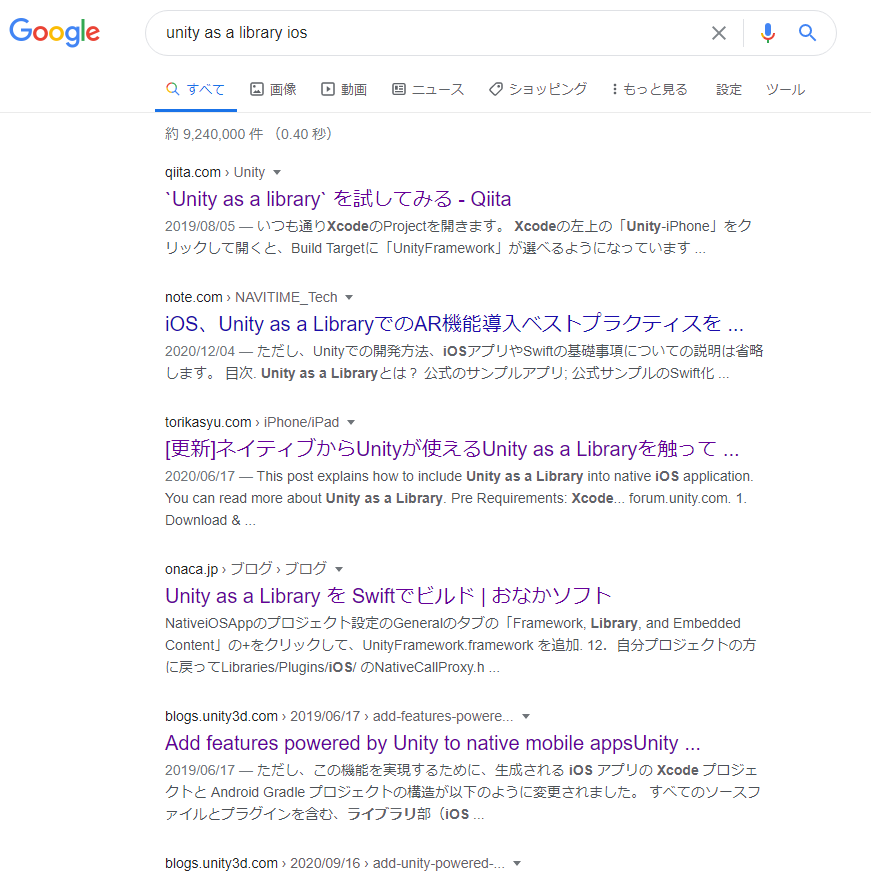
\includegraphics[width=60mm]{images/search-google.png}}
    \end{center}
    \caption{Google の検索結果一覧画面}
  \end{minipage}
  \begin{minipage}{0.5\hsize}
    \begin{center}
      \fbox{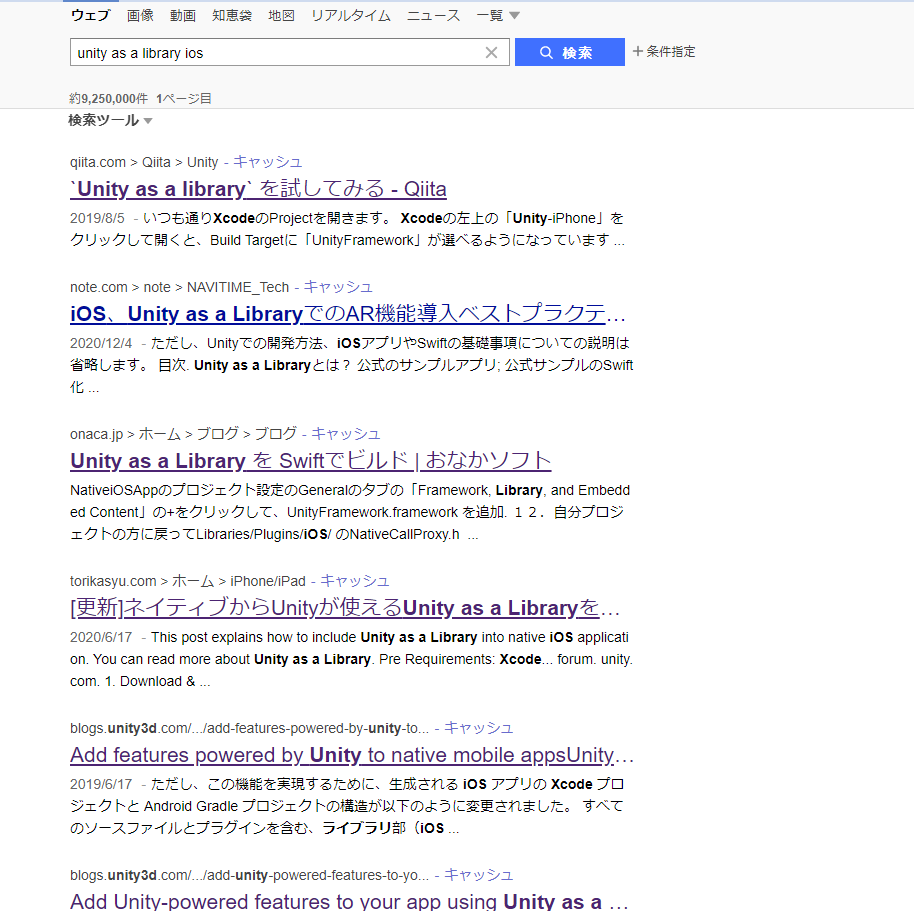
\includegraphics[width=60mm]{images/search-yahoo.png}}
    \end{center}
    \caption{Yahoo! の検索結果一覧画面}
  \end{minipage}
\end{figure}
\begin{figure}[htbp]
  \begin{minipage}{0.5\hsize}
    \begin{center}
      \fbox{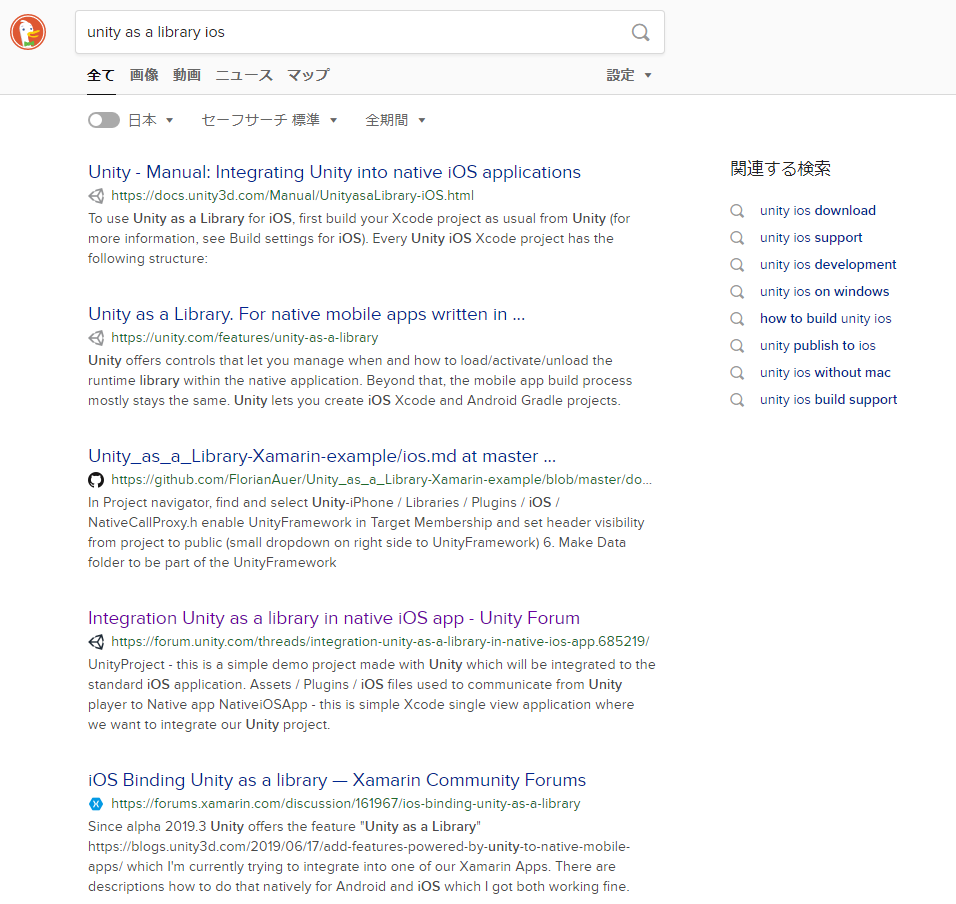
\includegraphics[width=60mm]{images/search-ddg.png}}
    \end{center}
    \caption{DuckDuckGo の検索結果一覧画面}
  \end{minipage}
  \begin{minipage}{0.5\hsize}
    \begin{center}
      \fbox{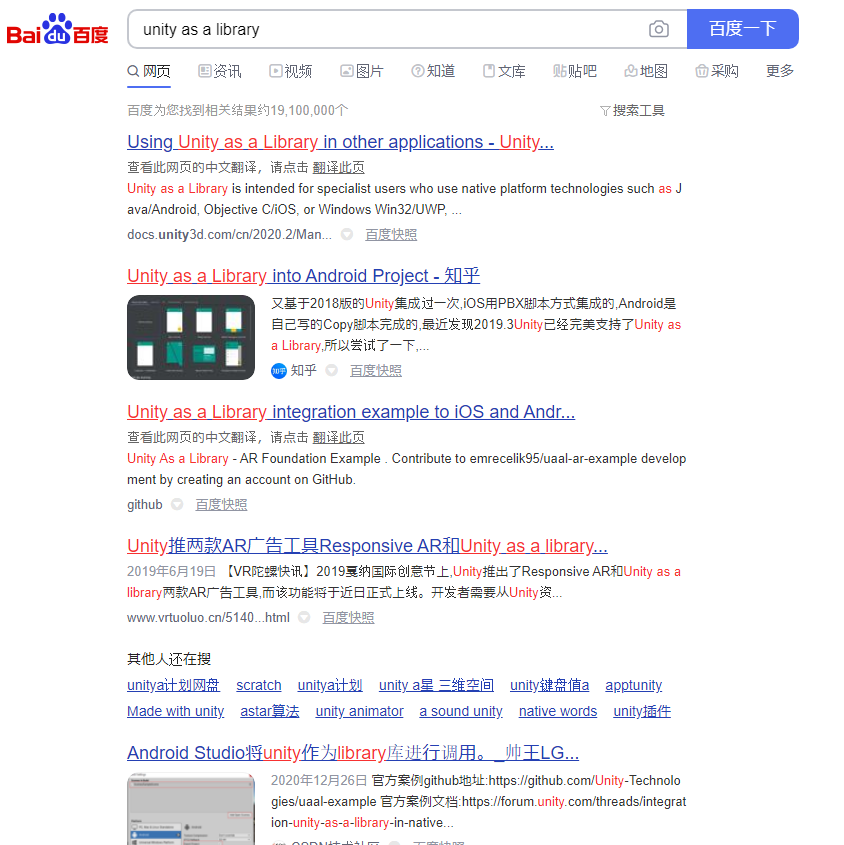
\includegraphics[width=60mm]{images/search-baidu.png}}
    \end{center}
    \caption{Baidu の検索結果一覧画面}
  \end{minipage}
\end{figure}

そこで,本来外見的な劣化のない各情報に,時間経過による表示の変化を与える.これにより情報の鮮度を直感的に認識できるようになり,Web 検索による情報収集を効率的に行えると考えた.

% こういった Web 検索結果一覧画面での情報の視覚化に関して,松下らは「ネット上の情報を可視化する技術」\cite{tecvisinfo}で,

% \begin{quote}
%   Web の規模が膨大になるにつれ,ランキングの精度がますます大きな問題となるが,精度向上にも限界があるため,情報可視化システムにかかる期待も今後大きくなると予想される.
% \end{quote}

% と述べている.

% また,ユーザが検索結果から最初の選択をするまでにかける時間が平均5.7秒だという調査\cite{pinball}があり,この短い時間でユーザに情報の鮮度を認識させなければならない.

リンク先のページの鮮度に応じてリンクの表現を変化させる「廃れるリンク」\cite{dyinglink}のようなシステムも存在するが,リンクのみへの適用であるため鮮度の表現方法に改善の余地があると考えた.

\section{本研究の目的}

本研究の目的は,ユーザがより直感的に情報の鮮度を認識できるように,ブラウザにおける検索結果一覧画面の表示を拡張することである.

\section{本文書の構成}

第\ref{chap:introduction}章では本研究における背景と目的について述べる.

第\ref{chap:verification}章では実際に視覚化システムを開発する前に様々な視覚化の方法を試し評価する.

第\ref{chap:implementation}章で開発したシステムの実装に関して述べ,第\ref{chap:discussion}章では実際に利用して得られた評価や今後の展望について述べる.

第\ref{chap:survey}章では本研究と関連のある研究事例を紹介している.第\ref{chap:conclusion}章では本研究を総括して結論を述べる.
	% 本文1
\chapter{鮮度の表現方法の検証}
\label{chap:verification}

本章では、情報の鮮度の視覚化について様々な視覚化の方法を試し、それぞれ考察していく。

以下で検証する全ての項目に関して図\ref{fig:ver-base}を利用する。

\begin{figure}[htbp]
  \begin{center}
    \fbox{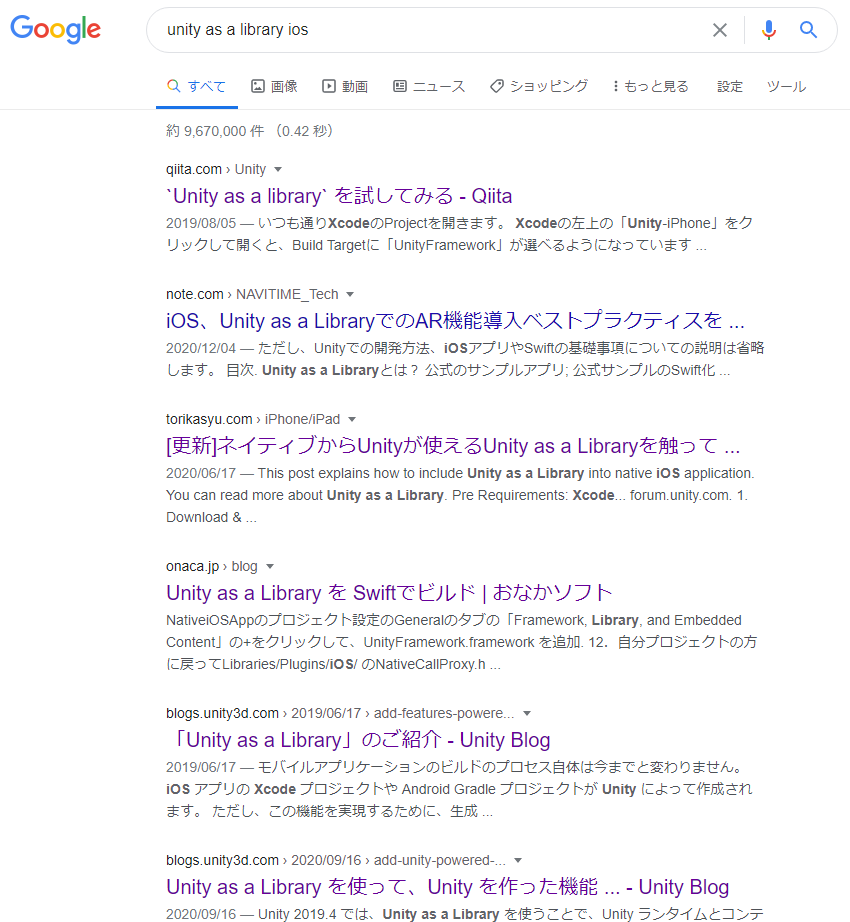
\includegraphics[width=60mm]{images/base.png}}
  \end{center}
  \caption{視覚化前の検索結果一覧}
  \label{fig:ver-base}
\end{figure}


\section{テクスチャによる変化}
\label{sec:ver-texture}

テクスチャを適用することで鮮度を視覚化する方法を検証する。

\subsection{紙の経年劣化}
\label{subsec:ver-tex-sheet}

実世界に存在する記録媒体で劣化するものを考えたときに最初に思い浮かんだのが紙である。

紙は時間が経つと黄ばみやシミができる。そういった変化を参考に、情報の鮮度を視覚化した。

\begin{figure}[htbp]
  \begin{minipage}{0.5\hsize}
    \begin{center}
      \fbox{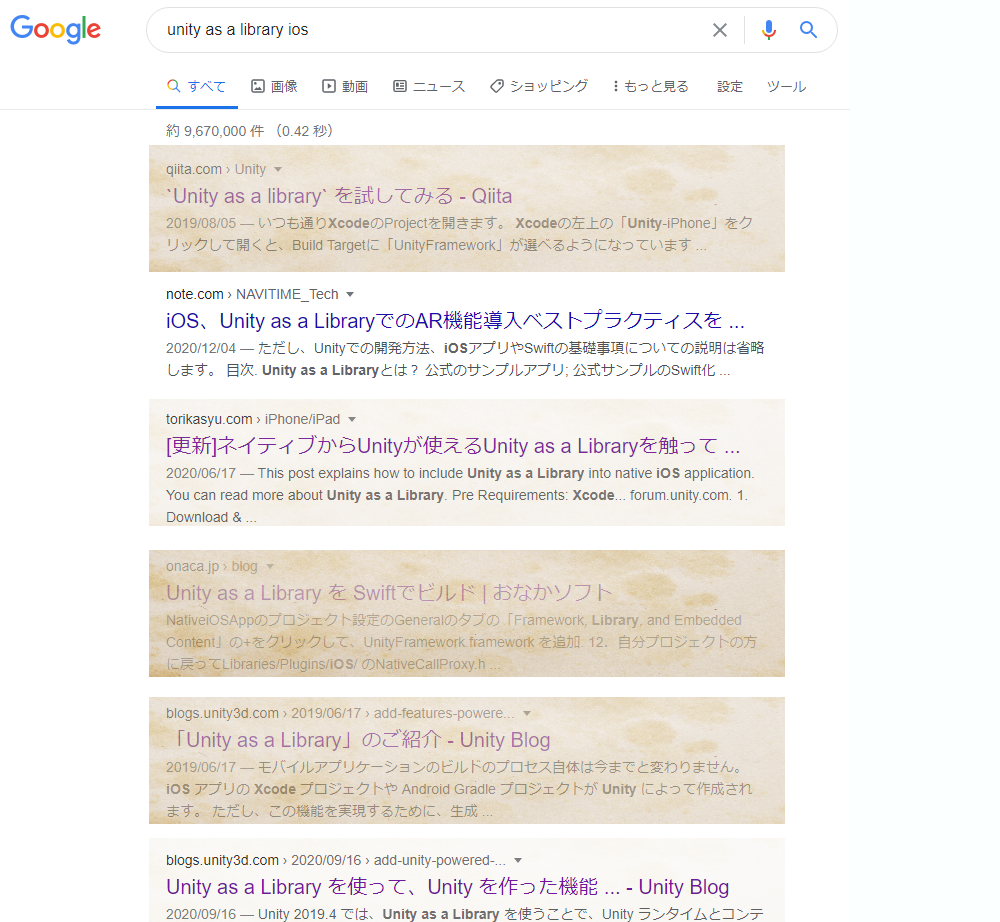
\includegraphics[width=60mm]{images/sheet-degradation1.png}}
    \end{center}
    \caption{紙の経年劣化をイメージした視覚化1}
    \label{fig:ver-sheet1}
  \end{minipage}
  \begin{minipage}{0.5\hsize}
    \begin{center}
      \fbox{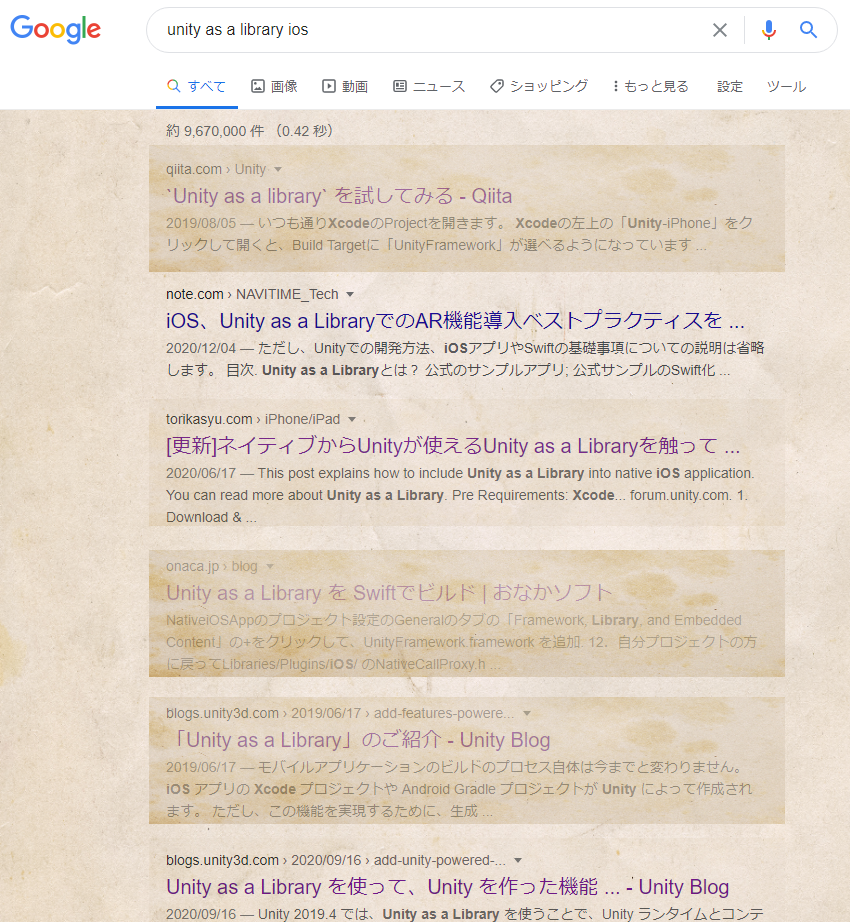
\includegraphics[width=60mm]{images/sheet-degradation2.png}}
    \end{center}
    \caption{紙の経年劣化をイメージした視覚化2}
    \label{fig:ver-sheet2}
  \end{minipage}
\end{figure}

各検索結果ごとに公開日を参考に、劣化した紙のテクスチャを適用したのが図\ref{fig:ver-sheet1}である。

さらに、全体に紙のテクスチャを適用することで劣化した紙のテクスチャが背景になじむように調整したのが図\ref{fig:ver-sheet2}である。

紙の劣化を参考にしているためか、古いということが分かりやすい。家や図書館などで古くなった本を見た経験がある人ならば、紙の時間経過による劣化を連想しやすいのではないだろうか。

図\ref{fig:ver-sheet1}に比べて、図\ref{fig:ver-sheet2}の方が背景に紙のテクスチャを設定しているため劣化した紙のテクスチャに違和感が少ない。

\subsection{金属のさび}
\label{subsec:ver-tex-russet}

実世界に存在するモノで紙以外に外見的な劣化の参考になるものを考えたとき、次に浮かんだのは金属である。

金属は雨風にさらされることでさびが発生するため、時間経過による劣化が簡単に見て取れる。これを参考に視覚化を行った。

\begin{figure}[htbp]
  \begin{minipage}{0.5\hsize}
    \begin{center}
      \fbox{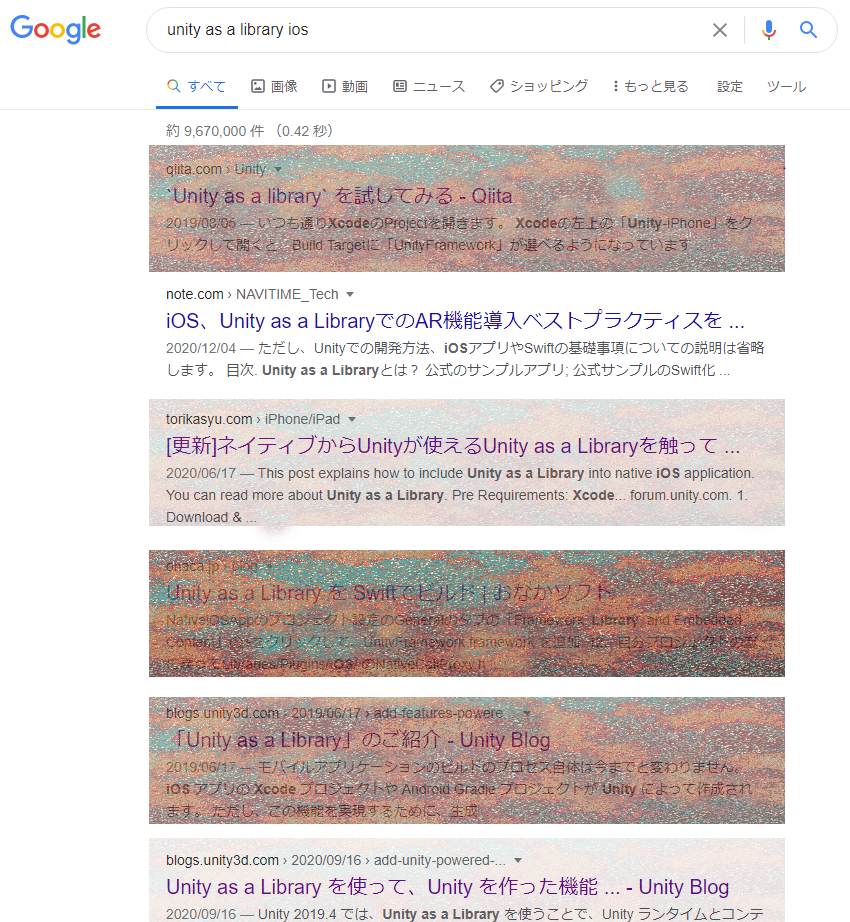
\includegraphics[width=60mm]{images/iron-russet1.png}}
    \end{center}
    \caption{金属のさびをイメージした視覚化1}
    \label{fig:ver-russet1}
  \end{minipage}
  \begin{minipage}{0.5\hsize}
    \begin{center}
      \fbox{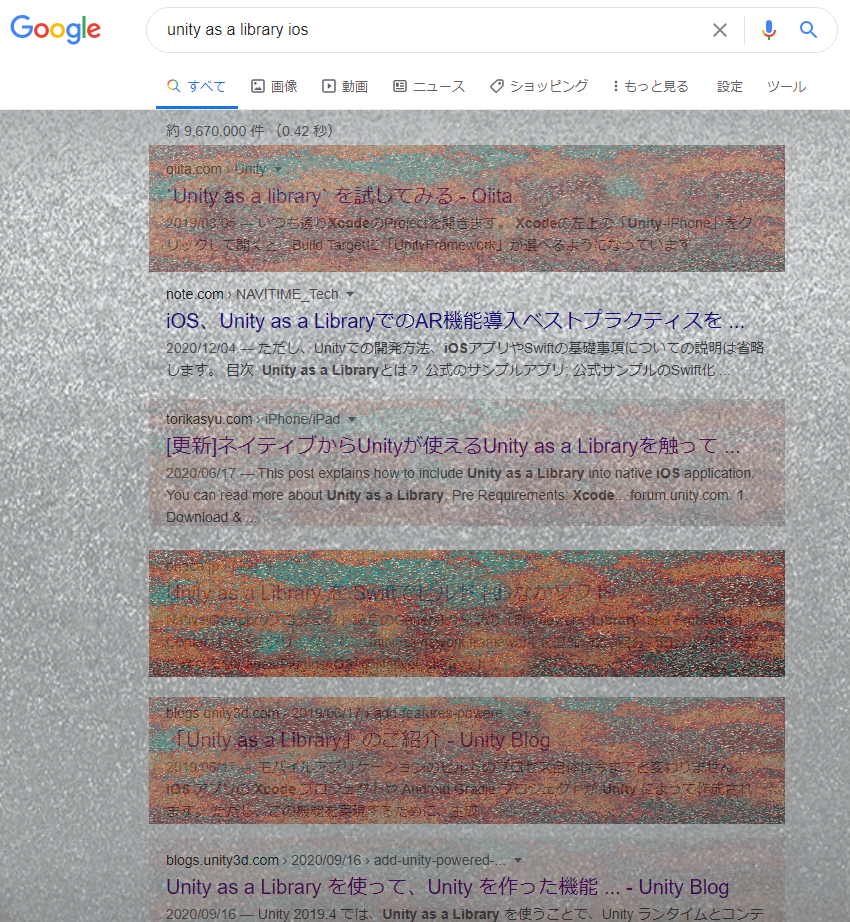
\includegraphics[width=60mm]{images/iron-russet2.png}}
    \end{center}
    \caption{金属のさびをイメージした視覚化2}
    \label{fig:ver-russet2}
  \end{minipage}
\end{figure}

\ref{subsec:ver-tex-sheet}の方法と同様に、錆びた金属のテクスチャを適用したのが図\ref{fig:ver-russet1}である。

また、背景に錆びていない金属のテクスチャを適用したのが図\ref{fig:ver-russet2}である。

\ref{subsec:ver-tex-sheet}と比べて古い情報が強調されているが、背景に金属のテクスチャを適用してもぬぐい切れない不自然さがある。

文字が記録されている媒体として金属があまり適していないことが原因と推測される。

\section{色による変化}
\label{sec:ver-color}

背景色や文字色を変更することで鮮度を視覚化する方法を検証する。

\subsection{背景の色褪せ}
\label{subsec:ver-col-cor}

実世界のモノが腐食するイメージを参考に、背景の色褪せによって情報の鮮度を視覚化した。

\begin{figure}[htbp]
  \begin{minipage}{0.5\hsize}
    \begin{center}
      \fbox{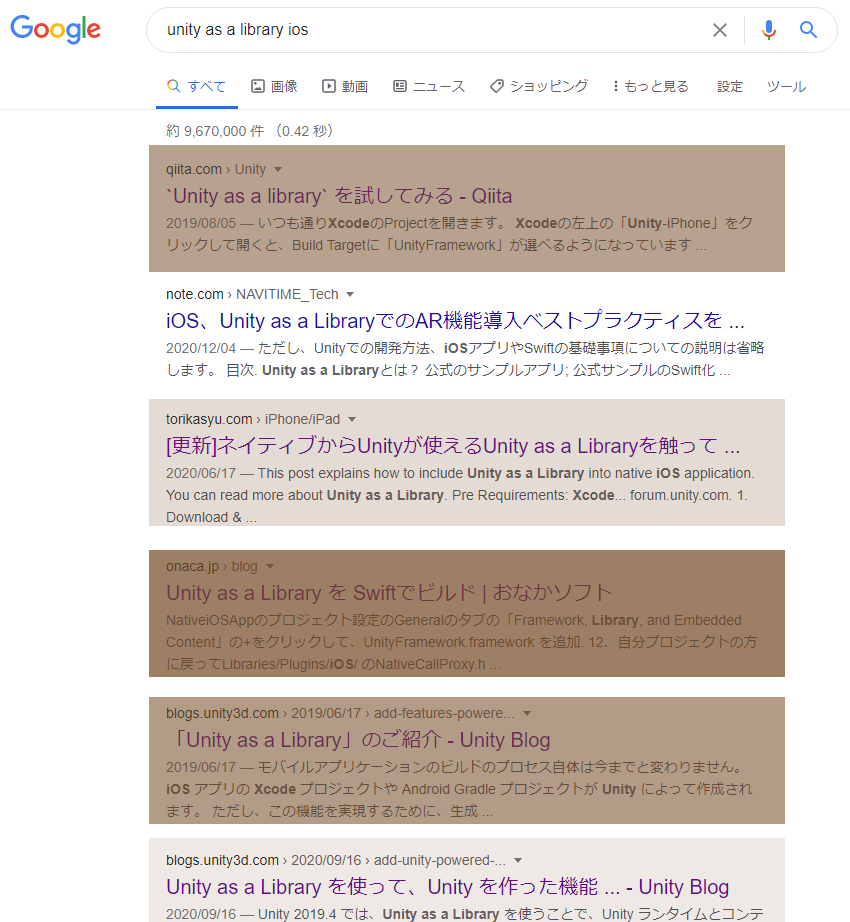
\includegraphics[width=60mm]{images/corrosion1.png}}
    \end{center}
    \caption{腐食をイメージした視覚化1}
    \label{fig:ver-corrosion1}
  \end{minipage}
  \begin{minipage}{0.5\hsize}
    \begin{center}
      \fbox{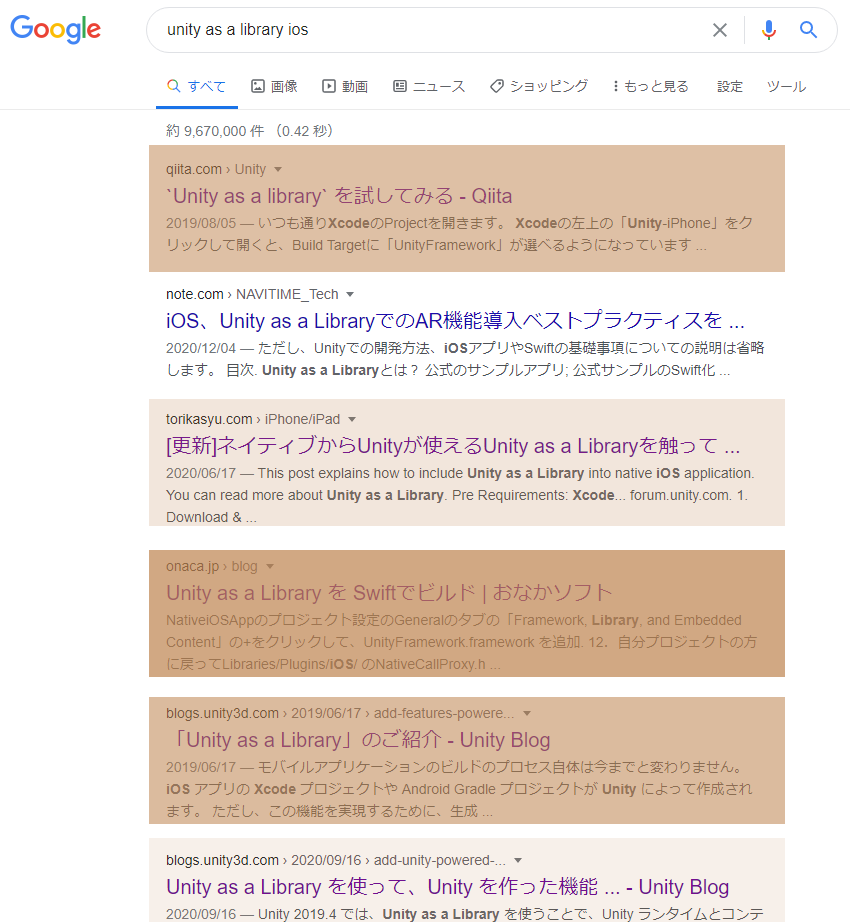
\includegraphics[width=60mm]{images/corrosion2.png}}
    \end{center}
    \caption{腐食をイメージした視覚化2}
    \label{fig:ver-corrosion2}
  \end{minipage}
\end{figure}

腐食を参考にしたため暗い茶色(図\ref{fig:ver-corrosion1})や赤茶色(図\ref{fig:ver-corrosion2})の中で鮮度ごとに色が変化するように、視覚化を適用している。

コンセプトとしては\ref{sec:ver-texture}で検証した二つと近いが、こちらの方がシンプルな分、元の白い背景に対して不自然さがないが、鮮度を示すものということが認識しにくい。

色の選定部分においては議論の余地があると考えられる。

\subsection{インクの劣化}
\label{subsec:ver-col-ink}

紙に書いた文字のインクが時間経過によって劣化していくのを参考に、情報の鮮度を視覚化した。

\begin{figure}[htbp]
  \begin{minipage}{0.5\hsize}
    \begin{center}
      \fbox{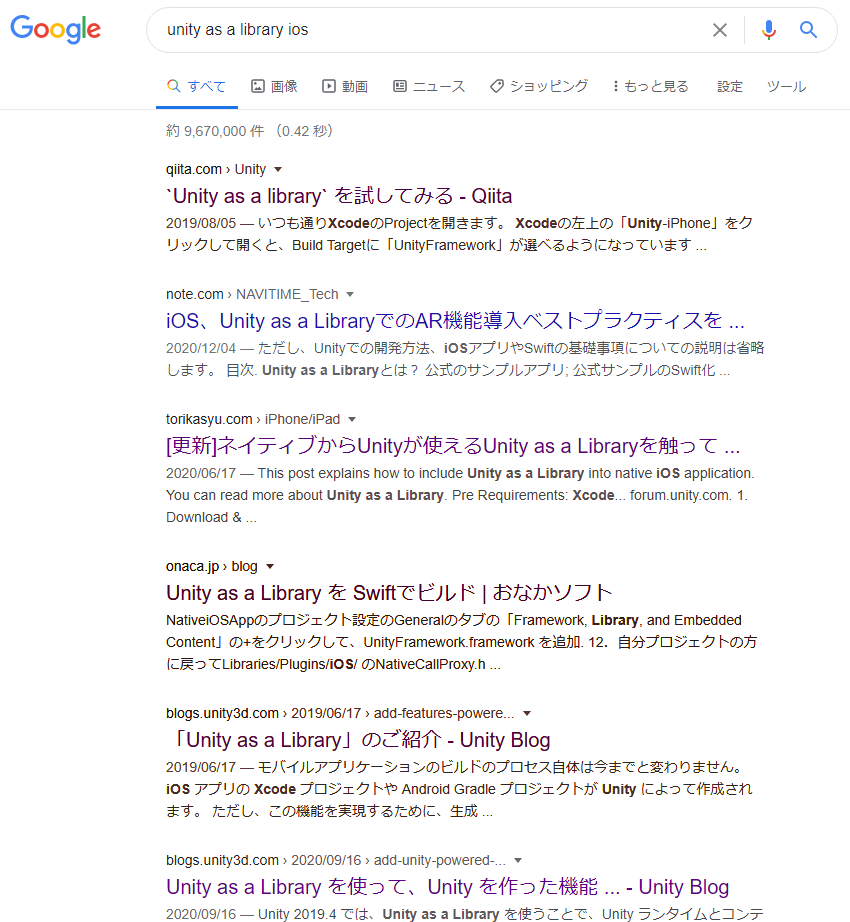
\includegraphics[width=60mm]{images/ink1.png}}
    \end{center}
    \caption{インクの劣化をイメージした視覚化1}
    \label{fig:ver-ink1}
  \end{minipage}
  \begin{minipage}{0.5\hsize}
    \begin{center}
      \fbox{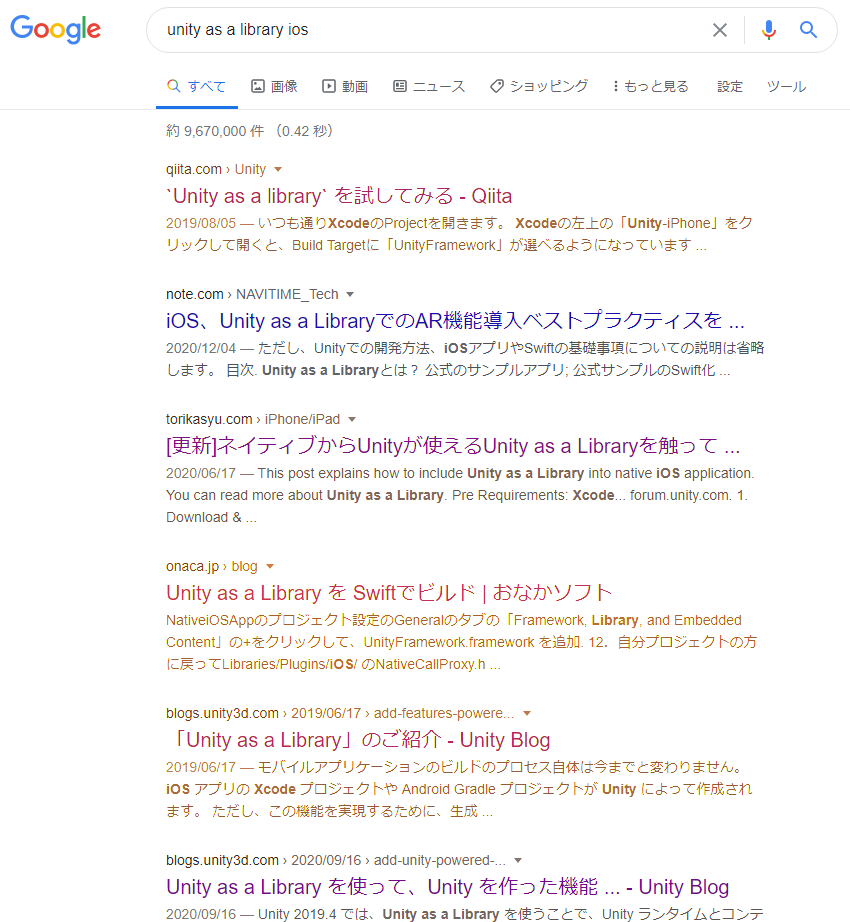
\includegraphics[width=60mm]{images/ink2.png}}
    \end{center}
    \caption{インクの劣化をイメージした視覚化2}
    \label{fig:ver-ink2}
  \end{minipage}
\end{figure}

\ref{subsec:ver-col-cor}と同様に、情報の鮮度に応じて文字の色が焦げ茶色に近づくようにしたのが図\ref{fig:ver-ink1}である。

また、背景色の白に薄まるように変化を加えたのが図\ref{fig:ver-ink2}である。

図\ref{fig:ver-ink1}に関しては、視覚化による変化が目立っておらずユーザに情報の鮮度を認識させるという目的が果たせていない。

図\ref{fig:ver-ink2}は、古い印象を与えることには成功しているが、古いか新しいかの二択に捉えられやすいと思われる。

どちらの場合も段階的な変化を認識しやすい視覚化の方法とは言えない。

\section{文字の消失による変化}
\label{sec:ver-character}

文字の一部、または全体を欠落させたり存在感を薄めることで鮮度を視覚化する方法を検証する。

\subsection{透明化}
\label{subsec:ver-chr-trp}

実世界のモノが時間経過によって消失していくさまをイメージして、各項目の不透明度を変更することで鮮度の視覚化を行った。

\begin{figure}[htbp]
  \begin{center}
    \fbox{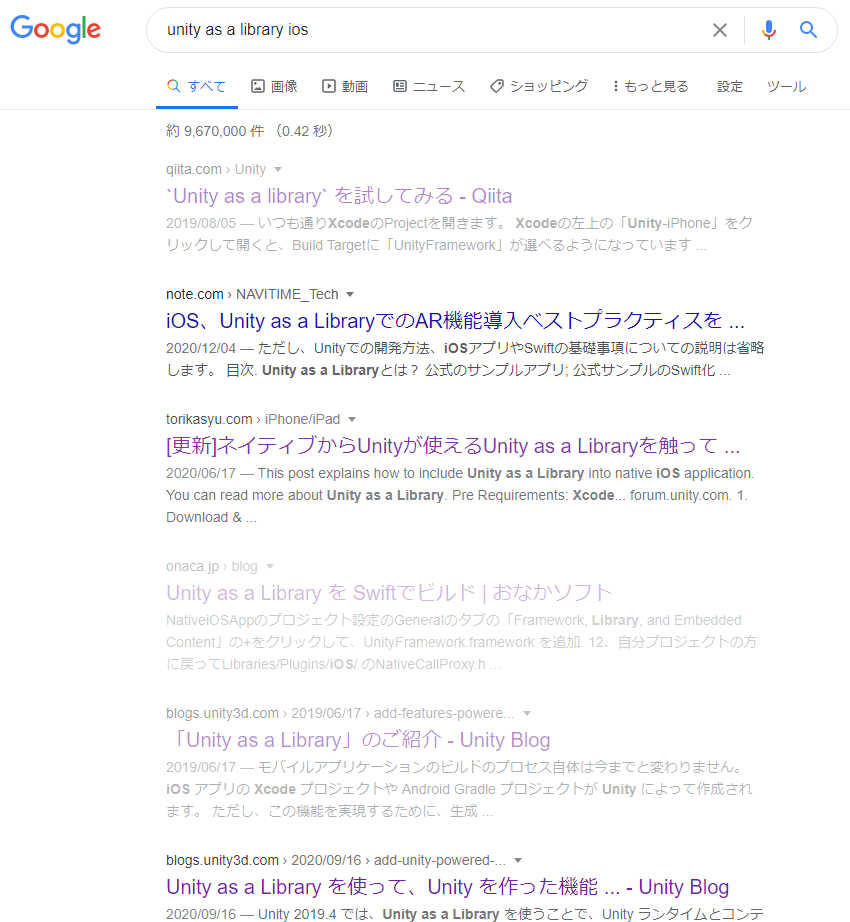
\includegraphics[width=60mm]{images/transparence.png}}
  \end{center}
  \caption{不透明度を変更した視覚化}
  \label{fig:ver-transparence}
\end{figure}

図\ref{fig:ver-transparence}は、各情報ごとに古いければ古いほど不透明度が下がっていくように視覚化を行ったものである。

元の検索画面に対して微小な変更のみを加えているため、不自然な点が少ない。また、段階的な変化が認識しやすく時間経過を簡単に見て取れる。

しかし薄いもの(不透明度が低いもの)が古いという結びつけが弱いため、鮮度を表しているという認識を与えられるか疑問がある。

\subsection{滲む}
\label{subsec:ver-chr-bld}

紙にインクをたらしたときにインクが滲んでいくイメージを参考に、鮮度を視覚化した。

\begin{figure}[htbp]
  \begin{center}
    \fbox{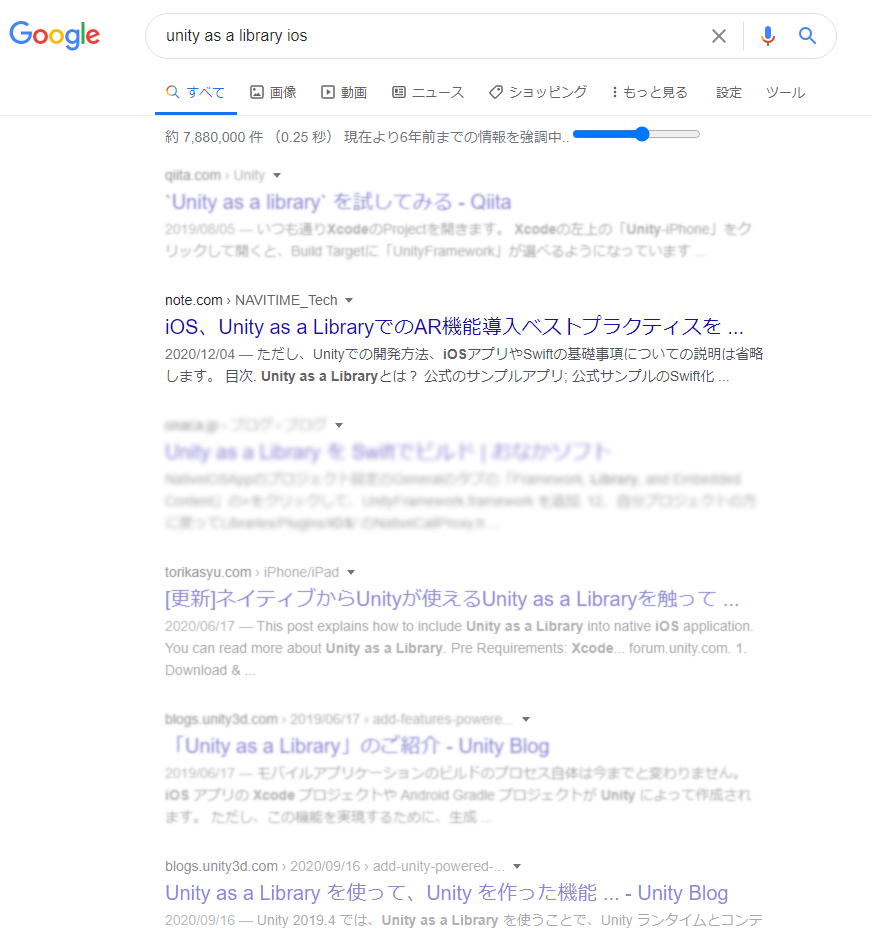
\includegraphics[width=60mm]{images/bleeding.png}}
  \end{center}
  \caption{インクの滲みをイメージした視覚化}
  \label{fig:ver-bleeding}
\end{figure}

\ref{subsec:ver-chr-trp}と同様の基準で、文字が滲むように変更を加えたのが図\ref{fig:ver-bleeding}である。

透明化のように元の背景とよくなじみ、段階的な変化が感じやすい。加えて、古いものを読ませないという効果も期待できる。

しかしながら、やはり滲んでいるから古い情報だという結びつけは弱いのではないだろうか。

\subsection{虫食い}
\label{subsec:ver-chr-wh}

古い書物などは紙自体の経年劣化の他にシミなどの虫による欠落が見られる。そういった劣化の仕方を参考に鮮度を視覚化した。

\begin{figure}[htbp]
  \begin{minipage}{0.5\hsize}
    \begin{center}
      \fbox{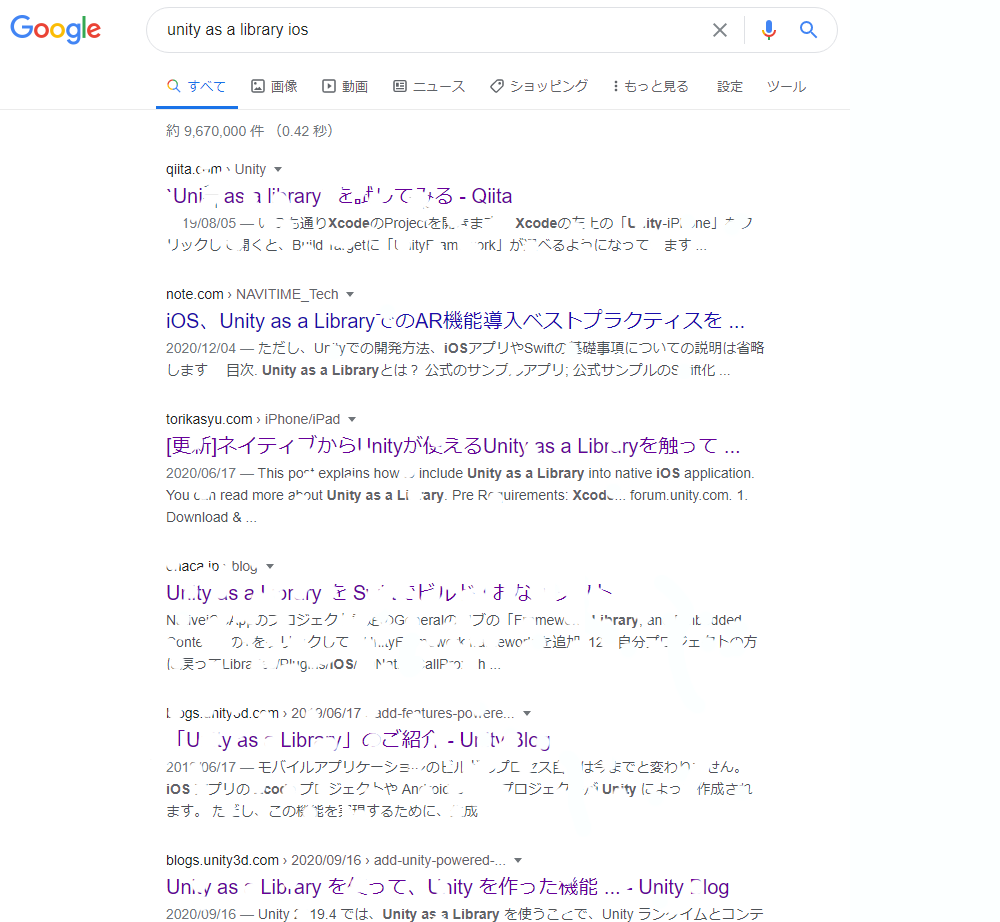
\includegraphics[width=60mm]{images/wormhole1.png}}
    \end{center}
    \caption{虫食いをイメージした視覚化1}
    \label{fig:ver-wormhole1}
  \end{minipage}
  \begin{minipage}{0.5\hsize}
    \begin{center}
      \fbox{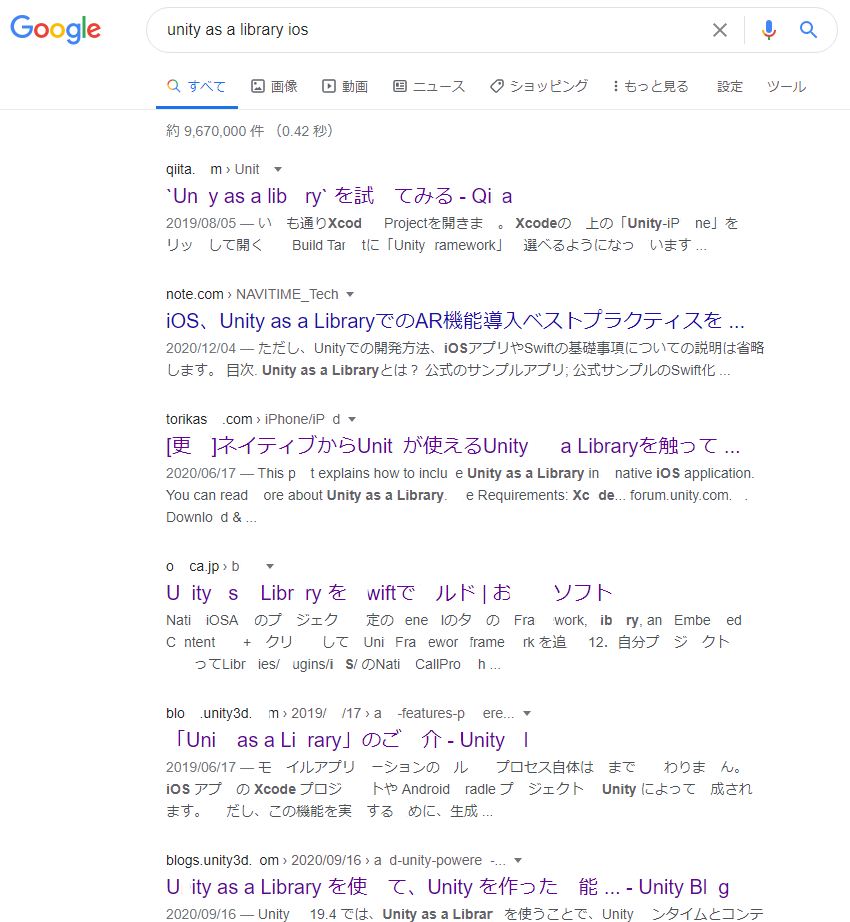
\includegraphics[width=60mm]{images/wormhole2.png}}
    \end{center}
    \caption{虫食いをイメージした視覚化2}
    \label{fig:ver-wormhole2}
  \end{minipage}
\end{figure}

図\ref{fig:ver-wormhole1}は実際に虫に食われた紙をイメージして、古いものがより欠損するように視覚化を行ったものである。

そして図\ref{fig:ver-wormhole2}は文章の虫食いをイメージして、古ければ古いほど多くの文字が欠落するように視覚化を行ったものである。

どちらも情報の鮮度に応じた変化の程度の差を設けるのが難しいが、古いものを読ませない効果は十分にあるだろう。

しかし、ある程度の文字が欠損していても何となくで読めてしまう部分があり、\ref{subsec:ver-col-ink}の視覚化と同様、段階的な変化ではなく読めるか読めないかの二分された認識になった。

\section{フォントによる変化}
\label{sec:ver-font}

使用されるフォントを変更することで鮮度を視覚化する方法を検証する。

\subsection{書体}
\label{subsec:ver-fnt-stl}

時代が進むごとに文字の書体も変わってきた\footnote{5分で学ぶフォントの歴史500年|時代背景とタイポグラフィ, https://note.com/smartcamp-design/n/n2740a3b72be9}。

古い情報は古そうだと感じられる書体を、新しい情報は新しそうだと感じられる書体を用いて記述することで情報の鮮度を視覚化した。

\begin{figure}[htbp]
  \begin{center}
    \fbox{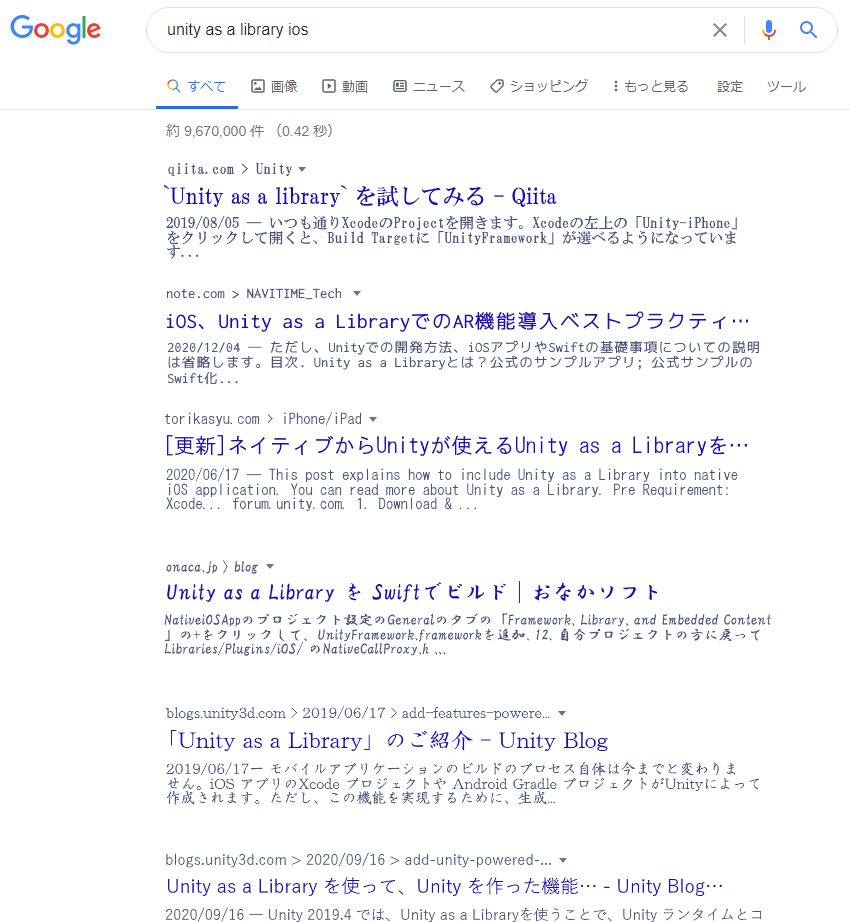
\includegraphics[width=60mm]{images/font-style.png}}
  \end{center}
  \caption{書体の変化による視覚化}
  \label{fig:ver-style}
\end{figure}

図\ref{fig:ver-style}は各情報ごとにWindowsに標準で搭載されているフォントを用いて、鮮度を視覚化したものである。

検証して分かったことだが、フォントの選定が難しく、人によって感じる印象が違うため鮮度を表すものとしては適さないと考えられる。

\subsection{ドット文字}
\label{subsec:ver-fnt-dot}

古い電子機器の画面ではピクセル数の関係からドット文字が使用されていたり、古さを演出するために意図的にドット文字を使うこともある。

そこで粒度の違うドット文字を用いて情報の鮮度を視覚化した。

\begin{figure}[htbp]
  \begin{center}
    \fbox{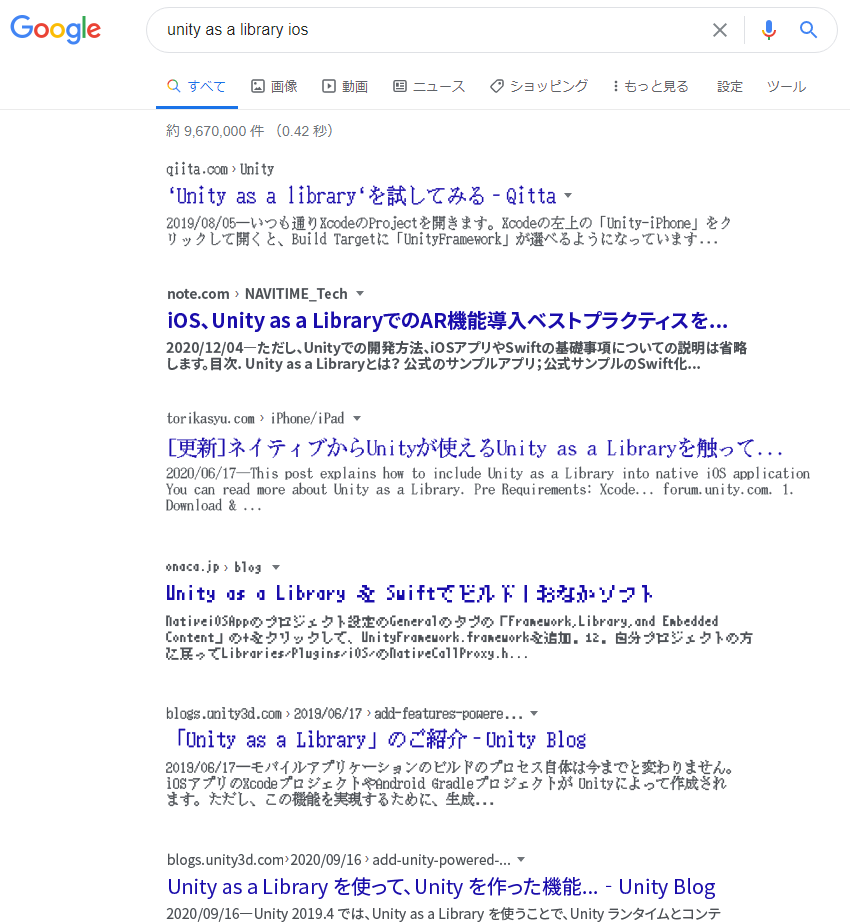
\includegraphics[width=60mm]{images/font-dot.png}}
  \end{center}
  \caption{ドット文字の粒度の変化による視覚化}
  \label{fig:ver-dot}
\end{figure}

古ければ古いほど粒度の荒いドット文字を使って表現したのが図\ref{fig:ver-dot}である。

予測では鮮度の段階ごとの変化を感じやすいと思われたが、古い印象よりも各サイトごとの特色だという印象の方が強かった。

これは各ドット文字がそれぞれ特徴的で、段階的な変化を感じさせなかったためだと推測される。

\section{その他の変化}
\label{sec:ver-other}

以上までに分類されない変化を用いて鮮度を視覚化する方法を検証する。

\subsection{テロメア}
\label{subsec:ver-oth-tlm}

Scrapboxというサービス\footnote{\url{https://scrapbox.io/}}内で用いられている、更新時刻を視覚化する機能\footnote{\url{https://scrapbox.io/shokai/%E3%83%86%E3%83%AD%E3%83%A1%E3%82%A2}}を参考に情報の鮮度の視覚化を行った。

\begin{figure}[htbp]
  \begin{center}
    \fbox{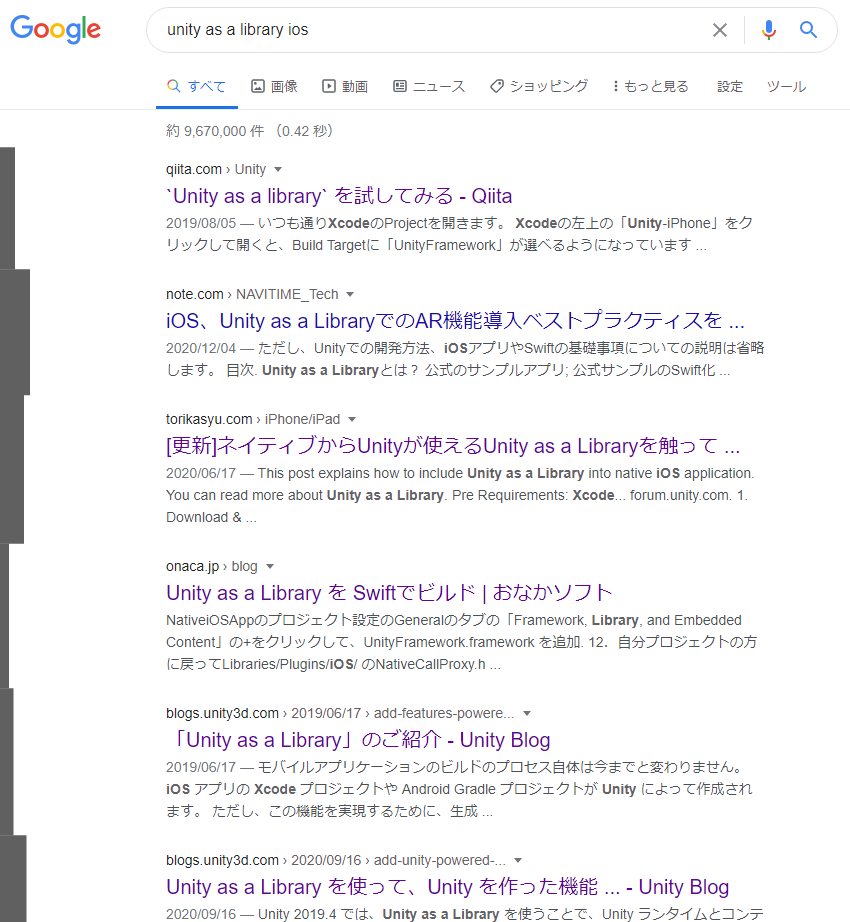
\includegraphics[width=60mm]{images/telomere.png}}
  \end{center}
  \caption{テロメアによる視覚化}
  \label{fig:ver-telomere}
\end{figure}

図\ref{fig:ver-telomere}は画面左端にテロメアを適用したものである。

各情報の鮮度ごとの段階的な変化が分かりやすく、それぞれの程度の差も直感的に感じられる。

しかし、同サービスを利用した経験がないユーザにはこれが情報の鮮度を表したものだと認識しにくいのではと推測される。

	% 本文2
\chapter{鮮度の視覚化の実装}
\label{chap:implementation}

本章では、第\ref{chap:verification}章で検証した鮮度の表現方法を参考に、実際にブラウザで動作する拡張機能の実装について述べる。

	% 本文3
\chapter{議論}
\label{chap:discussion}

本章では、第\ref{chap:implementation}章で開発した拡張機能を実際に運用した結果と評価について述べ、それを踏まえて議論を行う。

\newpage

\section{筆者の運用}

筆者は本拡張機能を開発段階から3か月程度利用した。利用している中で感じたのは、Web 上には古い情報が大量に存在しているということである。

新しい情報と古い情報がすべて均一に並べられていたという事実を今まで意識してこなかったことが痛感できた。また、全体を一覧した際にどの情報の鮮度がいいのかをすぐに識別可能で、新しい情報が欲しい際などにすぐに見つけることができた。

\section{第三者の意見}

研究会のメンバーの一人に本システムを実際に利用してもらい、フィードバックをもらった。

古いものが見えにくくなる点については、検索する分野によってはその分野の情報全体が古い場合があり、外見的な劣化が全体におよんでしまうという意見があった。

しかし同時に、情報の鮮度が視覚化されることによって通常の Web 検索に比べて、見ている情報の古さを意識できるようになったと評価された。

\section{関連研究}

廃れるリンク\cite{dyinglink}は Web 上のリンクに対して「モノが廃れる」メタファを適用することで、リンクの鮮度を一目で判断させること目的としたシステムである。

本研究との違いは、適用するメタファの選定や鮮度の算出部分の他に、こちらはブラウザにおける検索結果一覧に絞ったものという点である。

特に鮮度の算出に関して、廃れるリンクではプロキシサーバーを利用した大規模のものになっているが、本研究ではローカルの Chrome 拡張のみで動作することができるため、導入も容易である。

\section{今後の展望}

検証、実装および運用を経て、二つの問題点が浮かび上がった。

\begin{itemize}
  \item 情報の分野ごとに全体の鮮度の平均が違う
  \item 正確な情報の鮮度を取得できないことがある
\end{itemize}

それぞれに関しての考察と展望を以下に述べる。

\subsubsection{分野ごとの鮮度}

情報の分野によっては全体の鮮度が古い場合が存在する。例えば、既に更新が止まっている昔の技術を利用しようと検索をした場合、出てくる情報はいずれも古くなるのが必然である。

あるいは情報がすくない場合、一覧されるの情報の鮮度もバラツキが生まれ、外見的な劣化を加えることで本来よりも知りたい情報にたどり着きにくくなってしまう恐れがある。

そこでユーザが自由に、鮮度の算出を行う際の閾値を設定できるようにし、かつ、検索ワードごとの閾値のおススメを表示できるようにすれば、本システムの利点を残したまま、検索精度をあげることができる可能性がある。

\subsubsection{正確な鮮度の取得}

本システムでは検索結果一覧に並んでいる Google Chrome が表示している各項目の更新日時を参考にして鮮度を算出している。

しかし、Chrome の表示する更新日時は正確ではないこともあり、場合によっては表示されていないこともある。本システムでは更新日時が表示されていない情報に関しては、最も古いものとして扱っている。

他に更新日時を知る方法として該当リンク先のページで document.lastModified を実行して、時刻データを入手する方法がある。しかしこの方法はページの仕様によっては、コードを実行した時の時刻が返ってきてしまう。

筆者が調べた限りでは、現状全てのサイトごとの正確な鮮度を知る方法はなく、各サイトごとの更新者が申請する以外にない。それらを集めたデータベースなどを作る方法が考えられるが現実的とは言い難い。

この問題は今後の課題としたい。
	% 本文4
\end{verbatim}
\end{itembox}

目次に続いて、論文のメイン、本文を記述する。アブストラクトと同様で、{\tt main.tex}に直接書くか、\verb|\include| コマンドを利用して別に用意したファイルを{\tt include}する。

本文の書き方は、第\ref{chap:latex}章で詳しく説明する。


\subsection{謝辞の出力}

\begin{itembox}[l]{{\tt main.tex}}
\begin{verbatim}
\begin{acknowledgment}

本研究を進めるにあたり、ご指導いただきました増井井俊之先生に深く感謝いたします。

同じく、研究アイデアに対して多大なアドバイスをくださった左治木隆成氏をはじめとする増井研究会に所属している方々にも感謝の意を表します。ありがとうございました。

\end{acknowledgment}
	% 謝辞。要独自コマンド、include先参照のこと
\end{verbatim}
\end{itembox}

本文のあとには、謝辞を出力する。\verb|begin{acknowledgment}| から \verb|end{acknowledgment}| の間に書いた文章が、謝辞として独立したページに出力される。アブストラクトや本文と同じで、{\tt main.tex}に直接書いてもよいし、\verb|\include| コマンドを利用して{\tt include}してもよい。


\subsection{参考文献の出力}

\begin{itembox}[l]{{\tt main.tex}}
\begin{verbatim}

\begin{bib}[100]
% BibTeXを使う場合
\bibliography{main}

%\begin{thebibliography}{#1}
%
%  \bibitem{参照用名称}
%    著者名: 
%    \newblock 文献名,
%    \newblock 書誌情報,出版年.
%
% \bibitem{hoge09}
%   ほげ山太郎,ほげ山次郎:
%   \newblock ほげほげ理論のHCI分野への応用,
%   \newblock ほげほげ学会論文誌,Vol.31,No.3,pp.194-201,2009.
% 
% \bibitem{hoge08}
%   Taro Hogeyama, Jiro Hogeyama:
%   \newblock The Theory of Hoge,
%   \newblock {\it The Proceedings of The Hoge Society}, 2008.
%	
%\end{thebibliography}

\end{bib}
	% 参考文献。要独自コマンド、include先参照のこと
\end{verbatim}
\end{itembox}

謝辞に続いて、参考文献を出力する。

参考文献リストは、\verb|\begin{bib}| から \verb|\end{bib}| の間に、\verb|\bibitem| コマンドを使って書く。

BibTeXを使う場合は、以下のようにする。

\begin{itembox}[l]{{\tt 91\_bibliography.tex}}
\begin{verbatim}
\begin{bib}[100]
\bibliography{main}
\end{bib}
\end{verbatim}
\end{itembox}

こうすると、\verb|main.bib|から使用した参考文献のみを抽出して出力してくれる。\verb|main.bib|の中身は以下のようになっていて、気の利いた論文検索サイトであればBibTeXをコピペできるようになっているので簡単に作れるはず。


\begin{itembox}[l]{{\tt 91\_bibliography.tex}}
\begin{verbatim}
@article{hoge09,
    author  = "ほげ山太郎 and ほげ山次郎",
    yomi    = "ほげやまたろう",
    title   = "ほげほげ理論のHCI分野への応用",
    journal = "ほげほげ学会論文誌",
    volume  = "31",
    number  = "3",
    pages   = "194-201",
    year    = "2009",
}
@inproceedings{hoge08,
    author     = "Taro Hogeyama and Jiro Hogeyama",
    title      = "The Theory of Hoge",
    booktitle  = "The Proceedings of The Hoge Society",
    year       = "2008"
}
\end{verbatim}
\end{itembox}


以下は、BibTeXを使わないで手で書く例。

\begin{itembox}[l]{{\tt 91\_bibliography.tex}}
\begin{verbatim}
@article{hoge09,
    author  = "ほげ山太郎 and ほげ山次郎",
    yomi    = "ほげやまたろう",
    title   = "ほげほげ理論のHCI分野への応用",
    journal = "ほげほげ学会論文誌",
    volume  = "31",
    number  = "3",
    pages   = "194-201",
    year    = "2009",
}
@inproceedings{hoge08,
    author     = "Taro Hogeyama and Jiro Hogeyama",
    title      = "The Theory of Hoge",
    booktitle  = "The Proceedings of The Hoge Society",
    year       = "2008"
}
\end{verbatim}
\end{itembox}


英語の文献の場合、慣例的に書誌名をイタリック体にすることが多いらしい。

\begin{itembox}[l]{{\tt 91\_bibliography.tex}}
\begin{verbatim}
\begin{bib}[100]
\begin{thebibliography}{#1}
% \bibitem{参照用名称}
%   著者名: 
%   \newblock 文献名,
%   \newblock 書誌情報,出版年.

\bibitem{hoge09}
  ほげ山太郎,ほげ山次郎:
  \newblock ほげほげ理論のHCI分野への応用,
  \newblock ほげほげ学会論文誌,Vol.31,No.3,pp.194-201,2009.

\bibitem{hoge08}
  Taro Hogeyama, Jiro Hogeyama:
  \newblock The Theory of Hoge,
  \newblock {\it The Proceedings of The Hoge Society}, 2008.
\end{thebibliography}
\end{bib}
\end{verbatim}
\end{itembox}

\verb|\bibitem| コマンド中、参照用名称は、本文から参考文献を参照するときに使うので、忘れずに書いておく。参照文献を本文中に参照するときには、\verb|\cite{参照用名称}| のように書けばよい。例えば、この文の末尾には \verb|\cite{hoge09}| と書いてあるので、自動で対応する番号が振られる\cite{hoge09}\cite{hoge08}。

参考文献リストの番号付けと、本文で参照したときの番号の挿入は、全部が自動で行われる。ただしこれも、第\ref{sec:toc}節で説明した目次の出力と同じで、一時ファイルを生成してからの挿入なので、正しく出力するには最低でも二回のコンパイルが必要。BibTeXを使用する場合は、\verb|platex|コマンドのあと\verb|pbibtex|コマンドを実行し、さらに2回\verb|platex|コマンドを実行するといいらしい。



\subsection{付録の出力}

\begin{itembox}[l]{{\tt main.tex}}
\begin{verbatim}
\appendix
\chapter{付録の例}

付録を無理矢理出力させるため,てきとうなことを書く.

\section{ほげ}

コマンドは本文と一緒.

\subsection{ふー}

本文と一緒.

\section{ほげほげ}

本文と一緒.

\subsection{ふーふー}

本文と一緒.
		% 付録
\end{verbatim}
\end{itembox}

必要であれば、論文の最後には付録を出力する。

\verb|\appendix| コマンド以降に書いたものは、すべて付録として扱われる。付録部分の書き方は通常の本文とまったく同じで、\verb|\appendix| コマンド以降に書くだけで勝手に付録用の体裁で出力される。
